\section{Modeling}

\subsection{Motivation}
\enumstart
	\item Software is extremely complex
	\item A single programmer cannot manage this amount of code
	\item Code is not easily understandable by developers who did not write it
	\item Needs simpler representation for complex systems
\enumend

\subsection{Models}
\enumstart
	\item Abstraction of reality
	\item Abstraction from things, people and processes
	\item Relationships between these abstractions
	\item Simplification
	\enumstart
		\item ignore irrelevant details
		\item Relevance depends on purpose of model
	\enumend
	\item Goal - Manage and understand complicated systems through models
	\item Good Model
	\enumstart
		\item Intuitive - Relationships valid in reality are also valid in the model
	\enumend
\enumend

\subsection{Modeling Software}
\enumstart
\item Reality: Object-oriented software
\item Model: Diagrams that describe a software system from different points of view
\item Main purpose
\enumstart
	\item Sketch system before starting to implement
	\item Communication among developers
\enumend
\enumend

\subsubsection{UML - Unified Modeling Language}
\enumstart
	\item Recommended by Object Management Group (OMG)
	\item Defacto standard in industrial software development
\enumend

\subsubsection{Structural modeling}
\enumstart
	\item Class and object diagrams
	\item Identifying classes
	\item Mapping to code
\enumend

\subsubsection{Behavioral modeling}
\enumstart
	\item Sequence diagrams
	\item State machine diagrams
\enumend

\subsubsection{Class diagram}
\enumstart
	\item Most common UML diagram
	\item Shows types of objects and their static/structural relationships
	\item Classes:
	\tabularstart{|l*{1}{|c}}
		\hline
		Class name \\
		\hline
		Type Attribute \\
		\hline
		Signatur Operation\\
		\hline
	\tabularend
	\item Associations
		\tabularstart{l*{3}{c}}
			\tabularstart{|c*{1}{|c}}
				\hline
				Class \\
				\hline $\mathellipsis$\\
				\hline $\mathellipsis$\\
				\hline
			\tabularend
			\tabularstart{l*{3}{c}}
				multiplicity & Optional label & multiplicity\\
				\hline
				Optional role & & Optional role
			\tabularend
			\tabularstart{|c*{1}{|c}}
				\hline
				Class \\
				\hline $\mathellipsis$\\
				\hline $\mathellipsis$\\
				\hline
			\tabularend
		\tabularend
		\enumstart
			\item Class: Names the class...
			\item Multiplicity: Denotes how many objects the source object can reference
			\enumstart
				\item Exact number: $\{0,1,\mathellipsis\}$
				\item Arbitrary number: $\{*\}$
				\item Range: $\{e..f, e..*\}$ e,f mean exact numbers, $e < f$
			\enumend
			\item Label: In what kind of relation are the objects
			\item Role: What role does the source object have
		\enumend
	\item Qualified Associations
		\tabularstart{l*{3}{c}}
			\tabularstart{|c*{1}{|c}}
				\hline
				Class \\
				\hline $\mathellipsis$\\
				\hline $\mathellipsis$\\
				\hline
			\tabularend
			\tabularstart{l*{1}{|c}}
				\multicolumn{1}{c}{multiplicity}\\
				\hline
				Qualified Assoc.\\
				\hline
				\multicolumn{1}{c}{Optional role}
			\tabularend
			\tabularstart{l*{2}{c}}
				Optional label & multiplicity\\
				\hline
				 & Optional role
			\tabularend
			\tabularstart{|c*{1}{|c}}
				\hline
				Class \\
				\hline $\mathellipsis$\\
				\hline $\mathellipsis$\\
				\hline
			\tabularend
		\tabularend

	\item Navigability
	\\ 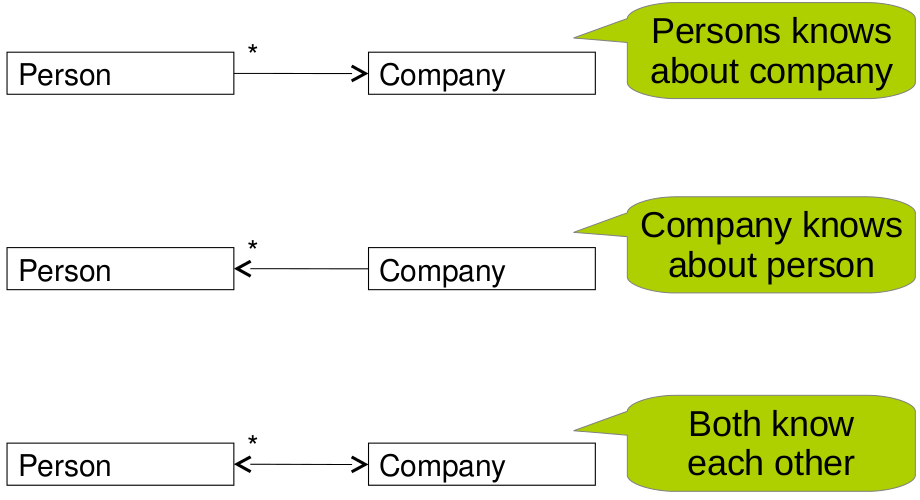
\includegraphics[width=0.5\textwidth]{img/association_directed.png}
	
	\item Aggregations
	\enumstart
		\item Variant of association
		\item Expresses a hierarchical part-of (has-a) relationship
		\item Classes can be part of several aggregates
	\enumend
	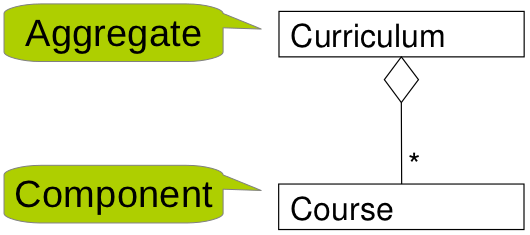
\includegraphics[width=0.5\textwidth]{img/aggregation.png}

	\item Composition
	\enumstart
		\item Expresses a strong aggregation
		\item No sharing of components
	\enumend
	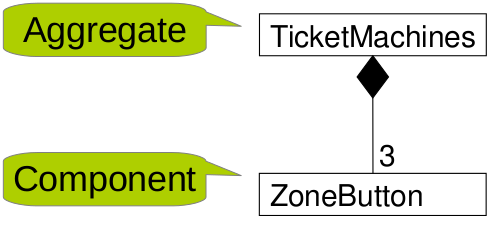
\includegraphics[width=0.5\textwidth]{img/composition.png}
	
	\item Generalization
	\enumstart
		\item Expresses a kind-of (is-a) relationship
		\item Implemented by inheritance
		\item Simplifies model by eliminating redundancy
	\enumend
	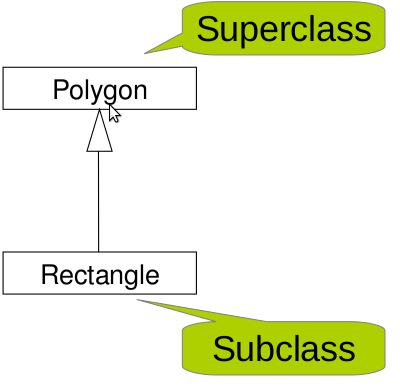
\includegraphics[width=0.5\textwidth]{img/generalization.png}
	
	\item Dependency
	\enumstart
		\item Express that changes to class B may cause changes to class A
		\enumstart
			\item A calls methods of B
			\item A mentions B as a parameter of a method
		\enumend
		\item Weaker then association, does not imply an attribute
	\enumend
	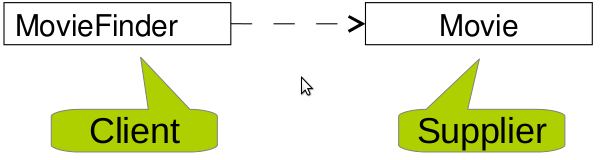
\includegraphics[width=0.5\textwidth]{img/dependency.png}
\enumend

\subsubsection{Object diagram}
\enumstart
	\item Shows snapshots of objects at a point in time
	\\ 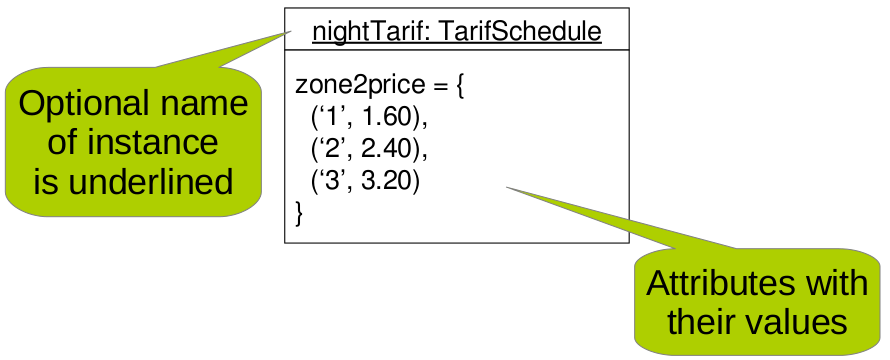
\includegraphics[width=0.5\textwidth]{img/object_diagram.png}
\enumend

\subsubsection{Identifying classes}
\enumstart
	\item Application domain approach
	\enumstart
		\item Ask application domain expert to identify relevant abstractions
	\enumend

	\item Syntactic approach
	\enumstart
		\item Extract participating objects from flow of events in problem statement
		\item Use noun-verb analysis to identify classes
		\enumstart
			\item Nouns: candidates for classes
			\item Verbs: candidates for operations
			\item Works well for short, structured text
		\enumend
	\enumend

	\item Design patterns approach
	\enumstart
		\item Use reusable design patterns
	\enumend

	\item Component-based approach
	\enumstart
		\item Identify existing solution classes
	\enumend

	\item Different kinds of objects
	\enumstart
		\item Entity objects
		\enumstart
			\item Represent the persistent information tracked by the system
			\item Application domain objects
			\item Changes rarely
		\enumend
		\item Boundary objects
		\enumstart
			\item Represent the interaction between the user and the system
			\item Changes very often
		\enumend
		\item Control objects
		\enumstart
			\item Represent the control tasks performed by the system
			\item Usually no concrete counterpart in the real world
			\item Changes often
		\enumend
	\enumend
	\item Stereotypes
	\enumstart
		\item Identifies the different kinds of objects in UML
		\\ 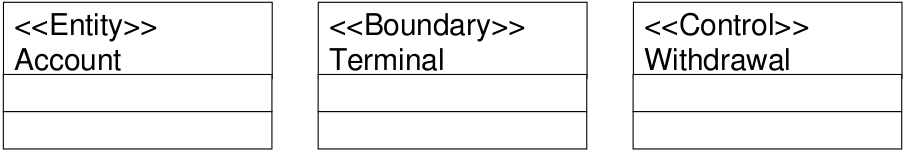
\includegraphics[width=0.5\textwidth]{img/stereotypes.png}
	\enumend
\enumend

\subsubsection{Mapping classes to code}
\enumstart
	\item Generalization
	\enumstart
		\item Inheritance
		\item Interfaces
	\enumend

	\item Visibility
	\enumstart
		\item Save connected objects as attributes
	\enumend

	\item Qualified association
	\enumstart
		\item Save a name for every connected object
		\item Probably use a dictionary datastructure
	\enumend

	\item Multiplicities
	\enumstart
		\item Ensure them by invariants
	\enumend
\enumend

\subsubsection{Sequence diagrams}
\enumstart
	\item Descripes operations of the class model
	\\ 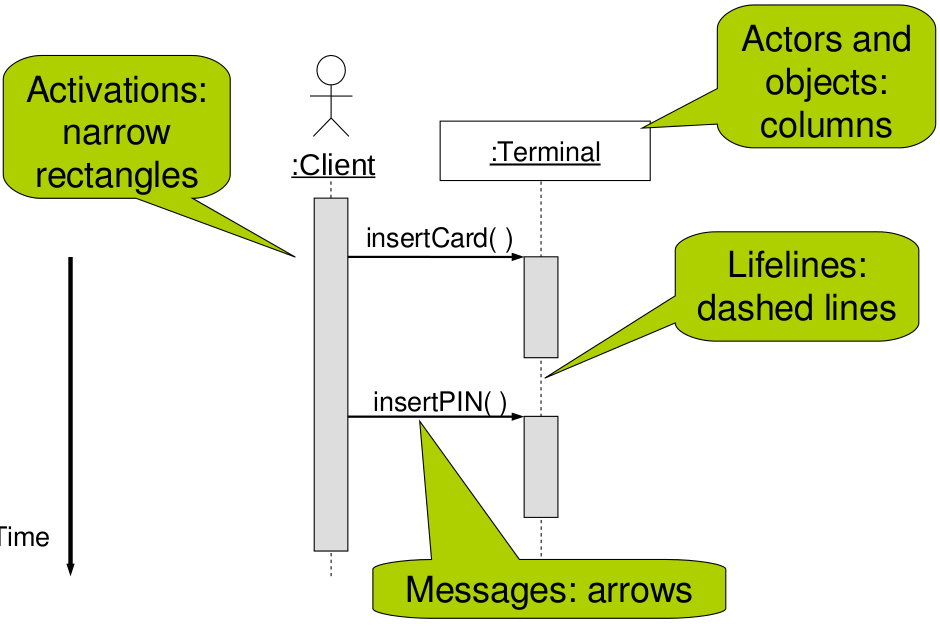
\includegraphics[width=0.5\textwidth]{img/sequence_diagram.png}

	\item Nested messages
	\\ 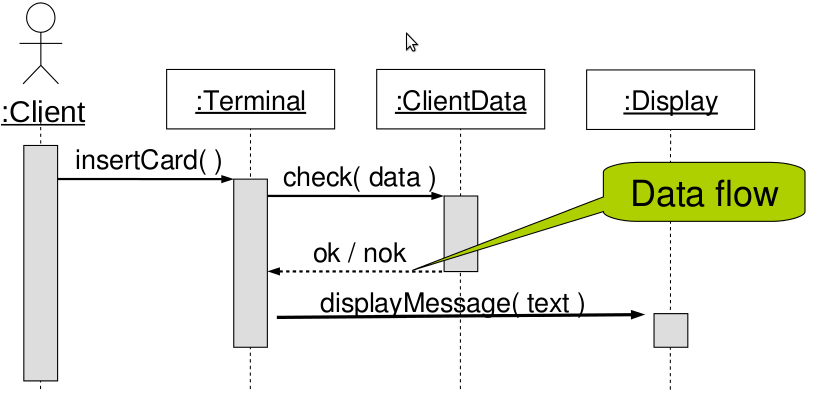
\includegraphics[width=0.5\textwidth]{img/nested_messages.png}
	
	\item Creation and destruction
	\\ 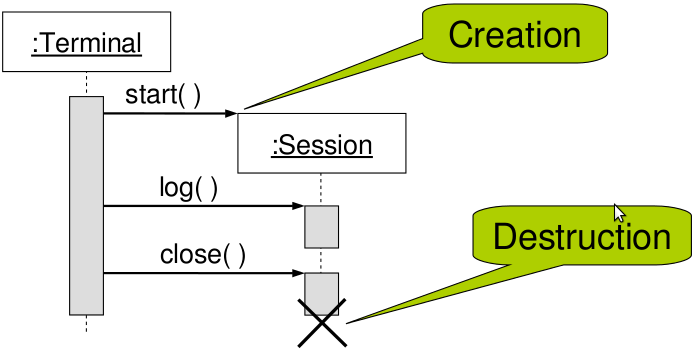
\includegraphics[width=0.5\textwidth]{img/creation_destruction.png}
	
	\item Recommended layout
	\\ 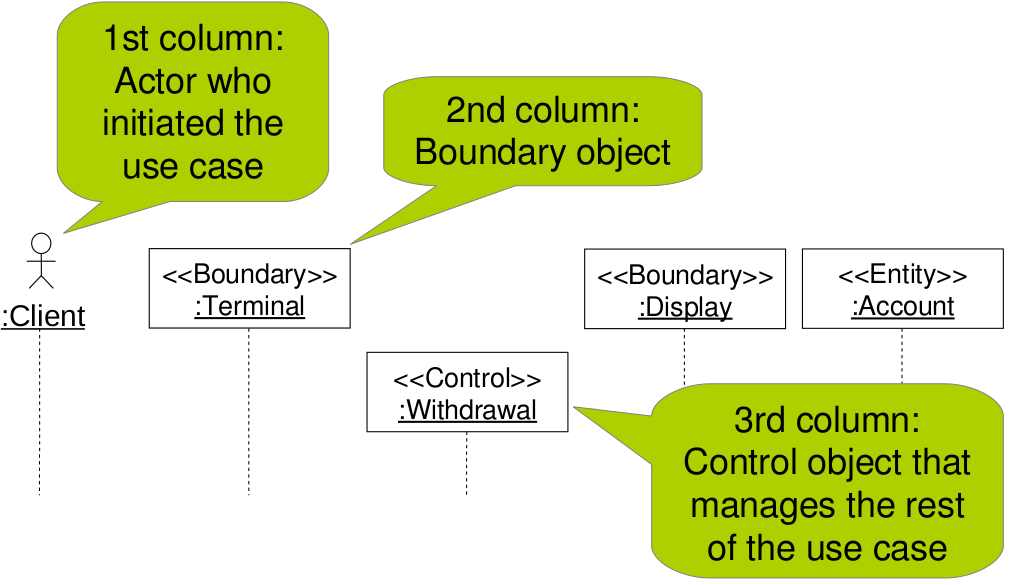
\includegraphics[width=0.5\textwidth]{img/recommended_layout.png}
	
	\item Heuristics for sequence diagrams
	\enumstart
		\item Creation of objects
		\enumstart
			\item Control objects are created at the initiation of the usecase
		\enumend
		\item Access of objects
		\enumstart
			\item Entity objects are accessed by control and boundary objects
			\item Entity objects never access control or boundary objects
		\enumend
	\enumend

	\item Structures
	\enumstart
		\item Fork structure
		\enumstart
			\item Dynamic behaviour concentrated in a single object
			\item Usually a control object
			\item Operations can change order
			\\ 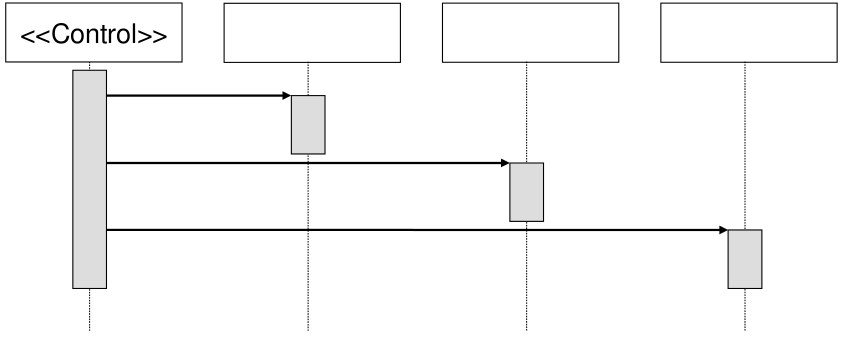
\includegraphics[width=0.5\textwidth]{img/fork_structure.png}
		\enumend
		\item Stair structure
		\enumstart
			\item Dynamic behaviour is distributed
			\item Objects delegate responsibility
			\item Chose when operations will always be performed in the same order
			\\ 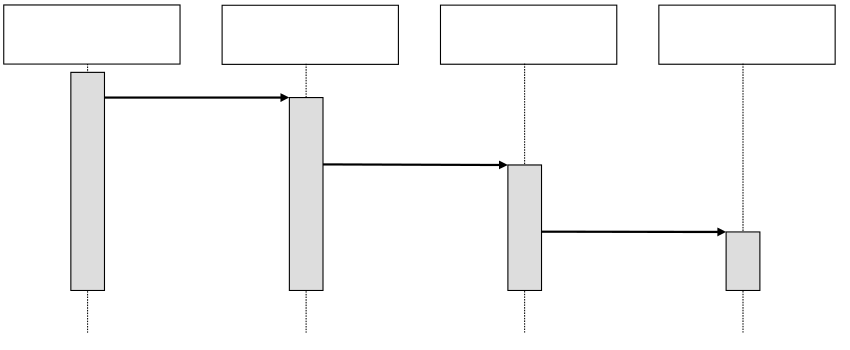
\includegraphics[width=0.5\textwidth]{img/stair_structure.png}
		\enumend
	\enumend
\enumend

\subsubsection{State machine diagrams}
\enumstart
	\item Long-living objects often have state-dependant behavior
	\enumstart
		\item Typical for control objects
		\item Sometimes also for entity objects
		\item Never for boundary objects
	\enumend
	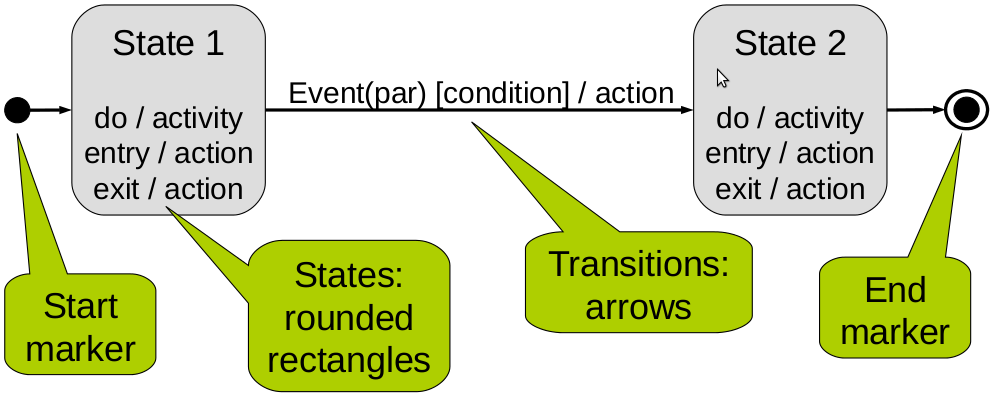
\includegraphics[width=0.5\textwidth]{img/state_diagram.png}
	\item Event: Something that happens at a point in time
	\item Action: Operation in response to an event
	\item Activity: Operation performed as long as operation is in some state
	\item Events can have different effects depending on guard conditions
	\\ 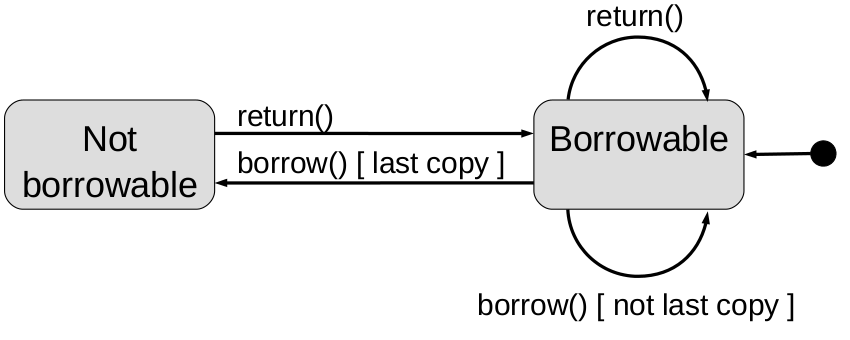
\includegraphics[width=0.5\textwidth]{img/guard_condition.png}
	\item Some state diagrams do not have end markers
	\item State diagrams can be nested (a state has its own state diagram)
\enumend

\subsubsection{Model-driven development}
\enumstart
	\item Idea: Work on the level of design models
	\item Generate code automatically (forward engineering)
	\item Advantages
	\enumstart
		\item Supports different implementation platforms
		\item Frees programmers from recurring activities
		\item Leads to uniform code
	\enumend
	\item Problems
	\enumstart
		\item Models may use different abstractions than programming language
		\item Models are incomplete specifications
		\item Models are informal
		\item Modification of generated code complicates things
	\enumend
	\item Reality
	\enumstart
		\item Mode-driven development is only a buzzword
		\item Code generation works only for very basic code
	\enumend
\enumend
